\chapter{What the matched simulations changed}
\label{vl:benchmark}

The virtual laboratory produced useful gains and useful failures. The important
comparison holds observations and acquisition cost fixed while changing the
inference or control design. The reported improvements apply to the specified
models and regimes; the controls prevent extrapolation to arbitrary hardware
or universally optimal experimental design.

\section{The first contrast loses to a stronger baseline}
The original curvature score and simultaneous probability box detect the
40-state driven-ring effect in only one of 200 held-out datasets, each with
50,000 records at each of three lags. A direct convexity contrast
$(-1,2,-1)$ detects it in 189 of the same datasets. This alone would be an
incomplete comparison: the fourth-edition numerical proposal routine can
optimize its scores and then check them over the entire continuous moment
class. That stronger box-based procedure detects all 200 datasets.

The result is retained. A more targeted confidence calculation does not
compensate for every weak choice of physical contrast. The simultaneous box
also permits score selection after acquisition, a flexibility the direct
single-contrast test does not share.

\section{A revised contrast succeeds at a smaller matched budget}
The second loop fixes the shifted-cubic contrast
$(-4/9,4/3,-1)$ before generating a newly seeded evaluation sample. It uses
5,000 independently simulated trajectory pairs per lag: 15,000 records and
4,500 units of expected evolution time per complete experiment. Both methods
receive exactly the same counts and settings. No pilot records are added for
this analytically chosen second-loop contrast.

\begin{center}
\begin{tabular}{lrr}
\toprule
Simulated case & Direct fixed contrast & Optimized moment-box method\\
\midrule
Driven ring & $367/400$ & $0/400$\\
Equilibrium ring & $0/400$ & $0/400$\\
Strong independent readout noise & $6/400$ & $0/400$\\
Common random-scale clock noise & $370/400$ & $0/400$\\
\bottomrule
\end{tabular}
\end{center}
The driven-case detection probability estimate is $91.75\%$, with a pointwise
95\% Clopper--Pearson Monte Carlo interval of $88.61$--$94.25\%$. Zero detections
in 400 equilibrium runs gives a corresponding upper interval endpoint of
$0.918\%$, not a proof of zero error probability. The theoretical false-positive
guarantee remains $5\%$ under the declared contract. Strong readout noise
remains a failure regime for useful power.

The revised certificate's mean entropy-rate lower bound in the driven case is
about $0.00115$, whereas the model's true rate is about $56.9$. The improvement
is in detecting a positive requirement at a finite budget, not accurately
recovering total dissipation. Neither reset energy nor detector/controller
energy is calibrated by this numerical model.

The comparison uses the implemented optimized-box procedure, whose numerical
search proposes scores and whose rational polynomial calculation verifies them.
A zero result alone does not prove that every possible score fails. We therefore
also construct exact equilibrium points inside the boxes. In 329 of the 400
driven datasets, a symmetric two-state model with a suitable fixed stochastic
detector lies inside the whole rectangular confidence region. In 296 of those
same datasets the direct-contrast certificate is positive.

There is no contradiction. A lower bound valid uniformly over each such
rectangle must allow its equilibrium point; the direct test uses a different,
predeclared confidence region. The countermodels establish a limitation of
that rectangular admissible set, rather than a universal limit on processing
the original counts. They rely on the stated unknown-detector-variance contract.
Independent zero-lag readout calibration could remove some of these alternatives.

\section{Sampling and calibration costs determine the recommendation}
For the original convexity contrast, reallocating the same 150,000 records from
$(50{,}000,50{,}000,50{,}000)$ to $(37{,}500,75{,}000,37{,}500)$ reduces the
concentration proxy. Expected evolution time remains 45,000 units. An
independent 200-dataset cohort gives 195 detections, compared with 189 in the
original cohort. Their Monte Carlo intervals overlap; this small difference is
not presented as a precisely established performance gain. The exact reduction
in the confidence proxy is the supported design statement.

The dependent-record experiment shows why favorable power is insufficient.
A stationary equilibrium model yields $24.7\%$ false equilibrium exclusions
under an unjustified independent-record calculation. A known mixing envelope
repairs coverage, but the supplied blind-gap design increases evolution time
from 1,800 to 3,601,800 units for the same record count. That large cost is part
of the result. An actual apparatus would need a justified faster reset, a
sharper dependence analysis, or a different observation protocol.

The dimension laboratory finds a complementary limitation. A coherent one
percent frequency error moves an intended oscillation minimum off the sampling
grid, reducing the old production protocol's power to $1.575\%$. One common
clock correction selected from an independent calibration sample restores
$98.72\%$ conditional production power. It preserves the classical common-
channel guarantee, but uses 260,000 additional pilot records. At an equal total
record budget, simple extra averaging beats the repair in some mild-noise
regimes; it fails to repair the larger phase offsets. Repeated use can amortize
calibration only while the apparatus remains stable.

\begin{figure}[p]
\centering
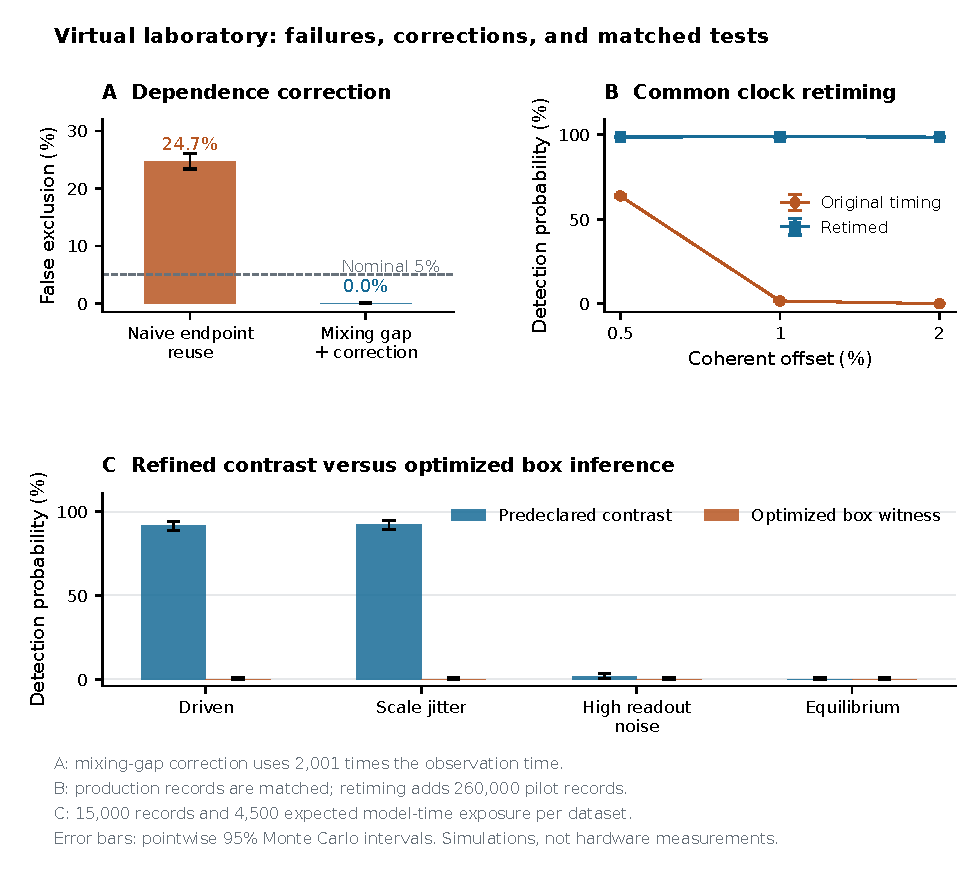
\includegraphics[width=\textwidth]{figures/virtual_laboratory.pdf}
\caption{Virtual-laboratory hardening under declared model and apparatus
contracts. Dependence corrections reduce false exclusions while increasing
sampling time. A common clock calibration repairs selected coherent-control
errors with an explicitly charged pilot. The lower panel compares the revised
fixed contrast and optimized moment-box procedure on identical 15,000-record
datasets. Error bars are pointwise Monte Carlo intervals. These are simulated
experiments; the panels have different access and cost contracts.}
\label{vl:summary-figure}
\end{figure}

\section{What is ready for physical transfer}
The transferable output is a procedure: specify the physical record, check
clock and exposure compatibility, justify conditional sampling envelopes,
freeze a targeted contrast or retain an exploratory joint region, and report
a certificate with its cost and failure controls. Exact simulator checks,
retained synthetic records and independent implementations make that procedure
inspectable by another researcher.

The next physical test should measure detector memory and exposure behavior,
validate stationarity or a preparation budget, and establish a time and energy
calibration before interpreting a positive bound. Matched comparisons should
include existing thermodynamic estimators when their required records are
actually available. The present endpoint-only experiments cannot establish
superiority over methods supplied with richer transition or waiting-time data.
Historical priority of the particular operational synthesis and physical
confirmation remain open.
